\section{Results \& discussion}
\label{sec:resul}
Due to each run of the experiment needing to spin up 30 docker containers and run Link State Protocol to convergence to generate routing tables,
each simulation took a lot of compute and ran for approximately 3 minutes. As such, the experimental surface plot was smoothened using a linear interpolating technique
to generate more plot points. Also, each experiment was only run once per setting of redundancy factor and packet drop rate, and further, due to randomness in graph generation, there are some 
outliers in the graph. 

\begin{figure}[ht]
    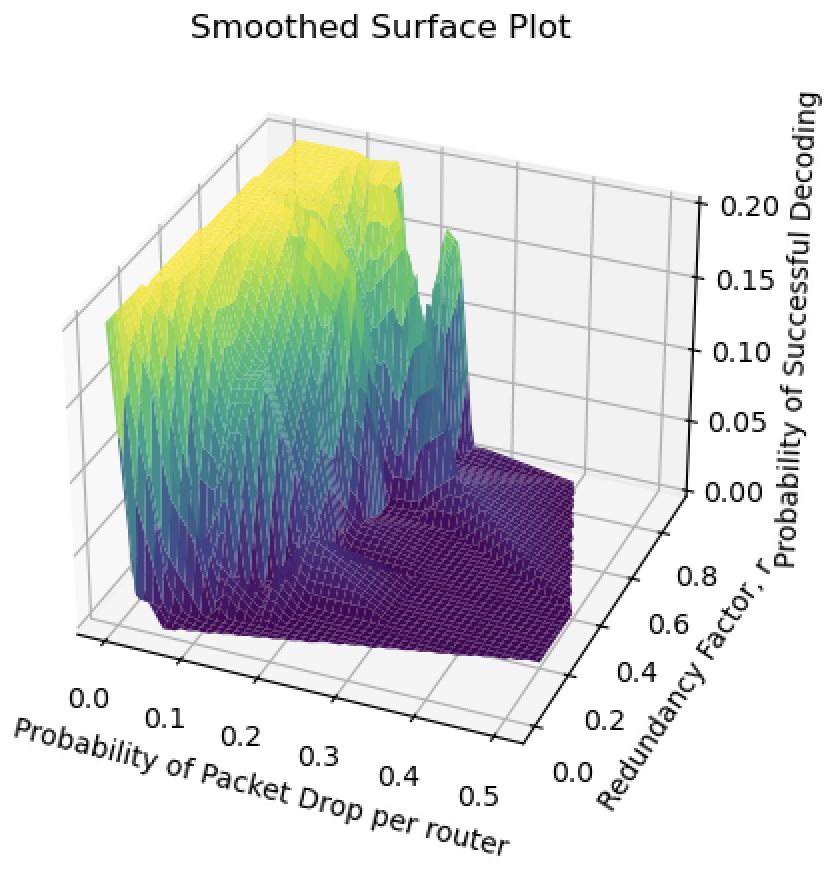
\includegraphics[width=0.48\textwidth]{experimental.png}  % Replace 'filename.ext' with your image file.
    \caption{Experimental Surface Plot=}  % Optional: add a caption.
\end{figure}

Nonetheless, we see that our surface plot roughly resembles the theoretical surface plot. We find that further work can be done to analyse the 
maximum of these surface plots, and a unconstrained optimization technique could be used to find the most suitable redundancy factor based on the unreliability of the particular network 
that a payload is about to be transferred over. 


\subsection{Theoretical Analysis}
Assuming that every router in the network has the same packet drop rate, we arrive at the following equations.
\begin{equation} \label{eq: yPlus}
    N = (1+\rho_{rf})*n
\end{equation}
where $N$ is the effective number of packets.
Further, defining $s$ as the survival per hop, we have 

\begin{equation} \label{eq: yPlus}
    s = 1-\omega
\end{equation}
In order for a packet to survive all hops, we have 
\begin{equation} \label{eq: yPlus}
    s_a = s^{h}
\end{equation}
where $h$ is the average number of hops taken by the packet thorugh the network. As such, we arrive at a final probability $p$ \\

\begin{equation} \label{eq: yPlus}
    p = \sum_{k=n}^{N}{N\choose k}s_a^k(1-s_a)^{N-k}
\end{equation}

Using this equation, we are able to plot the theoretical surface plot as shown.

\begin{figure}[ht]
    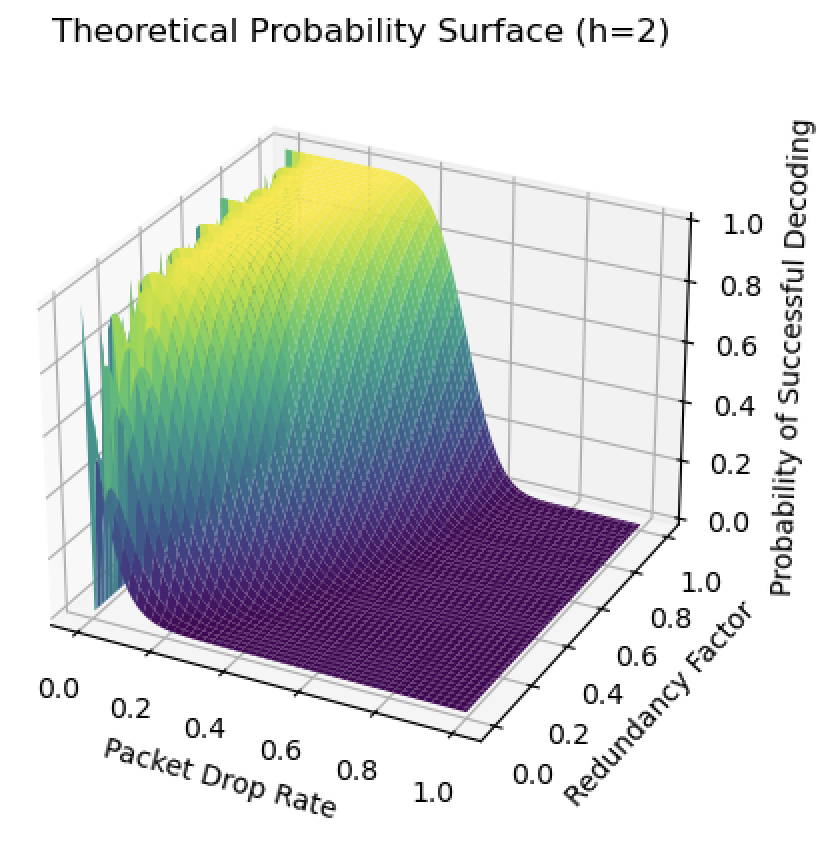
\includegraphics[width=0.48\textwidth]{2hops.png}  % Replace 'filename.ext' with your image file.
    \caption{Theoretical Surface Plot with h-2}  % Optional: add a caption.
\end{figure}

As we can see from the theoretical plot, as packet drop rate increases, the probability of a successful decoding decreases exponentially. 
This "unreliability" in the network can be offset by sending redundant packets as seen by the yellow surface in the plot. However, this only works to a certain extent, and when 
packet drop rates beyond 0.5 still result in a very low probability of successful decoding. It should also be noted that with larger payloads, the probability of a successful decoding could
be much lower. 




